\documentclass{sig-alternate}

\usepackage{times}
\usepackage{graphics}

\usepackage{subfigure}
\usepackage{booktabs}
\usepackage{colortbl}
\usepackage{tabularx}
\usepackage{color}
\usepackage{xspace}
\usepackage{hyperref}    % Creates hyperlinks from ref/cite
\hypersetup{pdfstartview=FitH}
\usepackage{graphicx}    % For importing graphics
\usepackage{url}         %

\hypersetup{%
pdftitle={Project Glass 2.0}, pdfauthor={Ben Zhang, Sean Chen}, pdfkeywords={HCI}, bookmarksnumbered, pdfstartview={FitH}, colorlinks,
citecolor=black, filecolor=black, linkcolor=black, urlcolor=black,
breaklinks=true,}

\renewcommand{\arraystretch}{1.2} % Space out rows in tables

\newcommand{\ml}[1]{{\color{green} {\it ML: #1}}}

% No space between bibliography items:
\let\oldthebibliography=\thebibliography
  \let\endoldthebibliography=\endthebibliography
  \renewenvironment{thebibliography}[1]{%
    \begin{oldthebibliography}{#1}%
      \setlength{\parskip}{0ex}%
      \setlength{\itemsep}{0ex}%
  }%
  {%
    \end{oldthebibliography}%
  }

%\pagenumbering{arabic}  % Arabic page numbers for submission.  Remove this line to eliminate page numbers for the camera ready copy

\begin{document}

% use this command to override the default ACM copyright statement
% (e.g. for preprints). Remove for camera ready copy.
%\toappear{Submitted for review to IPSN 2012.}
% \conferenceinfo{ConfName} {Date, Location}
% \CopyrightYear{Year} 
% \crdata{978-1-4503-1227-1/12/04} 
% \clubpenalty=10000 
% \widowpenalty = 10000


% to make various LaTeX processors do the right thing with page size
\special{papersize=8.5in,11in}
\setlength{\paperheight}{11in}
\setlength{\paperwidth}{8.5in}
\setlength{\pdfpageheight}{\paperheight}
\setlength{\pdfpagewidth}{\paperwidth}

\title{Project Glass 2.0 -- Interaction with Physical Devices through Attention}

\author{
{Ben Zhang, Sean Chen}\\
\affaddr{University of California, Berkeley}\\
%\affaddr{}\\
\email{benzh@eecs.berkeley.edu, sean.yhc@berkeley.edu}
}

\maketitle

\begin{abstract}
With the increasing interest of assigning intelligence to everyday object, many approaches of interacting with them fall back to smartphone based applications. We argue about the inconvenience, overhead, and distraction in such an interaction paradigm, and propose a more natural solution. A glass-based controller which enables user to express their interest in interaction directly simplifies the process of selection in a smart-home or smart-office senario. We present our thoughts, design and evaluation of such a system in this paper to motivate researchers in considering ``interaction in attention''. In the meantime, we noticed that Google Glass might serve as the perfect enabling technology, though in our prototype we've adopted infrared approach for proof-of-concept. The evaluation and discussion of such system might be valuable for future work to explore on more mature hardware platform.
\end{abstract}

%\category{C.2.1}{Computer-Communication Networks}{Network Architecture and Design}[Wireless communication]
%\keywords{Collection, CTP, Sensor Network, Routing}

% \category{B.0}{Hardware}{General}
% \category{B.4}{Hardware}{Input/Output \& Data Communication} 
% \category{H.4.m}{Information Systems Applications}{Miscellaneous}

% \terms{Design, Experimentation, Measurement} 
\keywords{HCI, Interaction, Attention, Infrared, Glass}

%!TEX root = sui14.tex
\vfill
\section{Introduction}
%\bjoern{We should see if we can change language in a few places to strengthen the connection to ``Spatial User Interaction", the title of the conference.}

%% from the swarm vision to the necessity of selection
The number of smart objects in our environment with embedded computation and communication has grown rapidly. These objects are all potential targets for interaction. To initiate {\em spatial interactions}, a user needs to first acquire the target object -- a fundamental task that has been extensively studied in graphical user interfaces, but not yet well-explored in {\em physical spaces}.

\changes{Today, companies like Samsung and Whirlpool are making smart appliances with companion applications that use smartphones as {\em universal remote controls}. With these applications, the user can select a device from a list in order to control it with a device-specific user interface. However, this method faces {\em naming} issues (i.e. ``what do we name the lamp on the left?'') and {\em scaling} issues as the number of controlled devices increases. These solutions also present a necessarily flawed mapping from the positions of the appliances in the rich, 3-dimensional world to their place in a 1D or 2D list presented on the screen. }
%
%% previous approaches are limited
Past research has used direct aiming at target devices in space with phones to overcome these problems~\cite{beigl_point_1999,patel_2-way_2003}. Such techniques have a few drawbacks: the aiming device first has to be retrieved; the user's hands have to be free for operation; and the user's visual attention is split between looking down at a screen and out at targets in the world. 

%% introducing head-worn computing and head orientation
Emerging head-worn computing devices do not require retrieval since the devices are already worn; they may enable hands-free or uni-manual interactions; and they offer near-eye or see-through displays to present information in the wearer's field of view. We thus investigate how such computing devices may be used for the selection and control of devices in physical spaces. Head-worn devices can naturally exploit the user's head orientation, an important (but imprecise) indicator of the user's {\em locus of attention}~\cite{raskin}. It suggests the general direction, but not the particular point of focus. We draw an analogy to assistive area cursors and adapt area cursor techniques~\cite{kabbash1995prince,worden1997making,findlater2010enhanced} for physical selection. Such techniques employ a two-step selection process: a {\em coarse} selection of an area of interest, followed by a {\em refinement} to select a target within that area.

In this paper, we describe the iterative development and evaluation of \systemnamenospace, an area-selection technique that can be readily implemented with small hardware changes to emerging head-worn devices. We augment Google Glass\footnote{\url{http://www.google.com/glass/start/}} to enable infrared (IR) communication between Glass and target appliances. We contribute and evaluate new methods for addressing selection ambiguity in this context. In all our techniques, the emitted IR beam %(a diameter of 30-60cm and distance up to 8m)%
 provides an initial {\em coarse} selection area (illustrated in Figure~\ref{fig:teaser} {\em left}). To {\em refine} selection when multiple targets have received IR signals, we describe and evaluate three techniques:

 Our {\em Naive IR} technique shows an alphabetically ordered disambiguation list on the near-eye display (Figure~\ref{fig:teaser} center). A study with $14$ participants finds that target acquisition with naive IR targeting is preferred by users and is faster than pure list selection without IR, but refinement is still time consuming.

Our {\em Intensity IR} technique improves refinement as target objects compare IR received signal strength (RSS). This value allows the system to eliminate some peripheral targets and to re-order the refinement interface's list by their intensity values. For example, in Figure~\ref{fig:teaser} of {\em Intensity IR} technique, device 5 is eliminated first and the list is re-ordered based on the intensity readings. A second study with $10$ participants shows that {\em Intensity IR} successfully reduces both the probability of needing to do refinement as well as the time spent in list navigation when compared to {\em Naive IR}.

Our final {\em Head-motion Refinement} addresses the lack of a natural mapping when users select a target in the refinement step using their device's touchpad --- the axes of motion do not map directly to the spatial layout of target devices in a room. We first learn the relative spatial structure of the targets using Glass' orientation sensors. Users can then perform head movements to change selections to spatially adjacent targets (see the right of Figure~\ref{fig:teaser}). For example, nodding down to select the target below current selection, or tilting right to select the next target on the right. We present preliminary feedback from participants on this technique.

We also demonstrate an example application of our technique used as a remote control of smart appliances such as lighting and TV sets: a user looks at the appliance he wishes to control and confirms selection by tapping. An appliance-specific user interface is then shown on the user's near-eye display for further interactions. 

%Orientation-based selection enables a wide range of context-aware applications. Examples include smart home remote control, break reminder monitor starer, museum attention tracking, indoor positioning, etc. In Figure\,\ref{fig:teaser}, it's a demonstration of the ``universal remote control'' scenario. The user can easily select the smart appliances by simply looking at it's general direction and confirm such selection with either voice command or by tapping the Glass input pad. Then an appliance-specific control UI will be shown on the head-mounted display. For this application, we have asked 14 participants to try the system and we report the qualitative results from them performing home automation tasks.


% In summary, this paper makes the following contributions:
% \begin{itemize}
% \item We presented our three iteractions of design.
% \item We present evaluations that compare head orientation targeting to list selection and quantify the benefits of automatic disambiguation.
% \item We demonstrate a home appliance remote control application built on top of our selection technique.
% \end{itemize}



%%% Local Variables: 
%%% mode: latex
%%% TeX-master: "sui14"
%%% End: 

\section{Related Work}
\label{sec:related-work}

In this section, we will first summarize some prior work and how it relates to our project in three folds: Tangible User Interface (TUI), Glass-based device, and Attention Aware System (AAS), discussing each in turn. 

\subsection{Tangible User Interface}
\label{sec:tang-user-interf}

The concept of Tangible User Interface was proposed in \cite{Ishii:1997:TBT:258549.258715}, and according to the original paper, such system would enable user to ``grasp \& manipulate bits in the center of users' attention by coupling the bits with everyday physical objects and architectural surfaces''. Thereafter, numerous TUI systems (such as \cite{Nanayakkara:2012:EEF:2212776.2212382, Patel:2006:IPA:2094945.2094962}) are developed. \cite{Merrill:2007:ALP:1758156.1758158} is one that is closest to our system, which base users' interaction with physical objects on people's natural looking, pointing and reaching metaphor. However, these systems have limitations that they focus too much on sensing the physical world, while the actuation is mostly done in cyber world. Recent years, many startups \cite{SmartThings, NinjaBlocks, Lockitron} tries to ``hack'' the physical world to achieve the envisioned Internet of Things by enabling actuating devices from phone/web portal. 

Our system combines some merits from prior work. We also user people's natural looking as attention tracking as in \cite{Merrill:2007:ALP:1758156.1758158}, but we are not limited to browsing or searching physical objects. We provide such capability of interacting directly with physical device, in addition to control with a mobile phone or web portal \cite{SmartThings, NinjaBlocks}.

\subsection{Glass Form-factor}
\label{sec:glass-form-factor}

\cite{mann2004continuous}, as the earliest wearable device, uses the form factor of glass to serve as a logging machine that records user's’ daily life. According to one review paper \cite{morris2010emerging}, there are many glass-based device developed for the past decades. Those who use glasses as input have primarily focused on gaze-tracking \cite{Selker:2001:EGE:634067.634176, Nagamatsu:2010:MDG:1753846.1753983}, and the projects that uses glasses for available output device works hard to achieve virtual reality \cite{Lumus, GoogleGlass}.

The most recent and potentially most impactful project \cite{GoogleGlass} integrate many crucial components -- camera, projection, microphone, speaker, IMU and networking -- into a single glass that can achieve virtual reality to an unimaginable extent. We do believe this might be a powerful platform for future interaction development. However, so far the vision is still being limited to Cyber world. Our project explores the potential of using glasses for direct interacting with physical devices, rather than doing ``digital'' tasks.

\subsection{Attention Aware System}
\label{sec:attent-aware-syst}

Microsoft Research's project ``Attentional User Interface'' \cite{horvitz2003models} explores how attention can be employed to enhance human-computer interaction, from the lesson learned in human-human interaction. Attention detection can also assist interface design to avoid context shifting overhead, e.g. the peripheral displays and the notification level should be adjusted according to user's attention \cite{parkdesigning}.

Our work also borrows ideas from these project in that we seek to identify users' attention to select the right physical object to interact.

%%% Local Variables: 
%%% mode: latex
%%% TeX-master: "main"
%%% End: 

\section{Design}
\label{sec:design}

% this section is used to discuss the design considerations of the system
% starting from a motivating example, and then extract the key requireements, then about system design

In this section, we will talk about our design considerations in solving the ``addressing'' problem in the smart environment. We start by describing the example application, where in an ideal case, how the user should interact with physical devices. From that, we draw some design requirements. To explore the design space, we propose several possible solutions. Some of them are difficult to achieve within a shrot time. In next section, we will build a proof-of-concept system, where we have simplified several tasks.

\subsection{Example Application}
\label{sec:example-application}

Our work is primarily motivated by the observation that in CS294-84 course at Berkeley, the instructor has to go to the switch to turn off the light during presentation. The separation of device and their controller makes it possible for people control things that are not reachable (such as the lights on the ceiling). However, such indirection introduces additional overhead since people still need to locate the controller and then interact. Remote control might mitigate such a problem, but one controller for one device is not a scalable solution. And squeezing controllers onto the smartphone display is also not the right approach. We will demonstrate this by giving the following Smart Home example.

% {\bf Smart Home}:
% Sean, maybe you can elaborate on this application more to motivate.
Imagine in a smart-home environment that most devices are remotely controllable. When the users are watching TV shows, they want to turn off the lights and turn up the volume so they can enjoy this memorable time. Such ordinary-life tasks are happening everyday, and any simplification will result in significant time savings. One ideal approach is that the user expresses his interest of turning off the lights by simply staring at the light, plus a specific gesture. Then he turns his head back to the TV, and again simply ``asks'' the TV to turn up the volume. When transitioning, the disconnection with the light and the connection with TV happens seamlessly, with the correct feedback for the user. And all the magic are resolved by an always-available device; this might be the glasses, rings or watches. 

Occasionally, the user needs to perform some advanced configurations to the TV, such as adjusting the white balance, or the brightness. Since the need of these complicated tasks are not frequent, and it will be less efficient to embed these features into the always-available device (which is designed to be small and easy-to-access, rather than too flexible). The smart-home falls back to a more generic approach which relies on touch screen or other rich input device. In this example case, since the user's attention is still on TV, his smartphone may pop up the control menu for advanced usage automatically. Such menu could also just pop up on walls or other large interactive displays \cite{unPad:eWallpaper, MSVision}. Even in this case, the attention system knows users' intention and saves time for user to address the device to interact.

\subsection{System Requirements}
\label{sec:system-requirements}

From what we have described in the previous section, the example application is enabled by a few necessary requirements. We will discuss some important ones in this section.

% leads to the adoption of glass
The first and foremost is the ability to sense and control in an always-available fashion. Since the goal is to simplify everyday task in a smart-home or smart-office scenario, any cubersome solution is not desired. The control of the device would also have to be simple, not to confuse the user of using it. 

Secondly, since screens might not always be available when users are interacting directly with physical device. Adequate feedback should assist user understanding what is going on. Even if screens are everywhere to assist in the future, the requirements of having proper feedback still hold.

As discussed before, we envision the simple always-available device would not be capable to cover all tasks. For those which are really complicated and less likely being executed, we will have to enable the system to fall back.

Besides the previous three, for any human-centric system, additional requirements like responsiveness would also be required, though not explicit discussed through this paper.

\subsection{System Design}
\label{sec:system-design}

In this section, we will present several design consideration that fulfills the requirements. From \cite{Merrill:2007:ALP:1758156.1758158}, they tried the solution of putting IR into earphones, rings to enable looking, pointing and reaching metaphor. When we were thinking about how to capture user's attention, we are actually leaning towards the glasses solution. Part of the motivation is from Google Glass. Generally, glasses are more natural in align with human's light of sight. Therefore, sensors on glasses can reflect the users' attention in a more precise way. Then given the glass form factor, what might be the right sensor or component to use to obtain users' attention remains a major question for us.

The first possible approach is a pure Google Glass solution. Since the glasses come with a camera, sophiscated computer vision algorithms might be able to detect what is in front of the user's sight. Following this thoughts, the camera would also be able to tell users' gestures. In fact, there are more features which would make this interaction cooler -- the voice recognition is another important source of user input, the projection onto user's eyeballs can provide timely feedback to users' action, the networking capability provide seamless connection with other peripheral devices such as displays. And initially, we were also thinking about building a prototype that resembles Google Glass, but the complexity behind of achieving acceptable image processing is huge. Not to mention we don't have the Google Glass yet. This approach is more an exploration of design space. 

Since our target is to validate the thoughts of interacting directly with physical objects through users' attention. We might break the initial proposal to several achievable tasks and build the proof-of-concept. Our second approach still adopts the glass form factor, but we've turned to other sensors to detect users' line of sight. 

Specifically, we choose to use IR. When surrounded by tubes, the IR is pretty directional. And from our test, it can differentiate objects in {\color{red} 20 (do some experiments here)} centimeters. User input can be captured by a slider on glass frame, where it's easy to access (though not hand-free). The networking capability is enabled by having an XBee module on the main board. We propose the interaction architecture in Fig.\,\ref{fig:sysarch}.

\begin{figure}
  \centering
  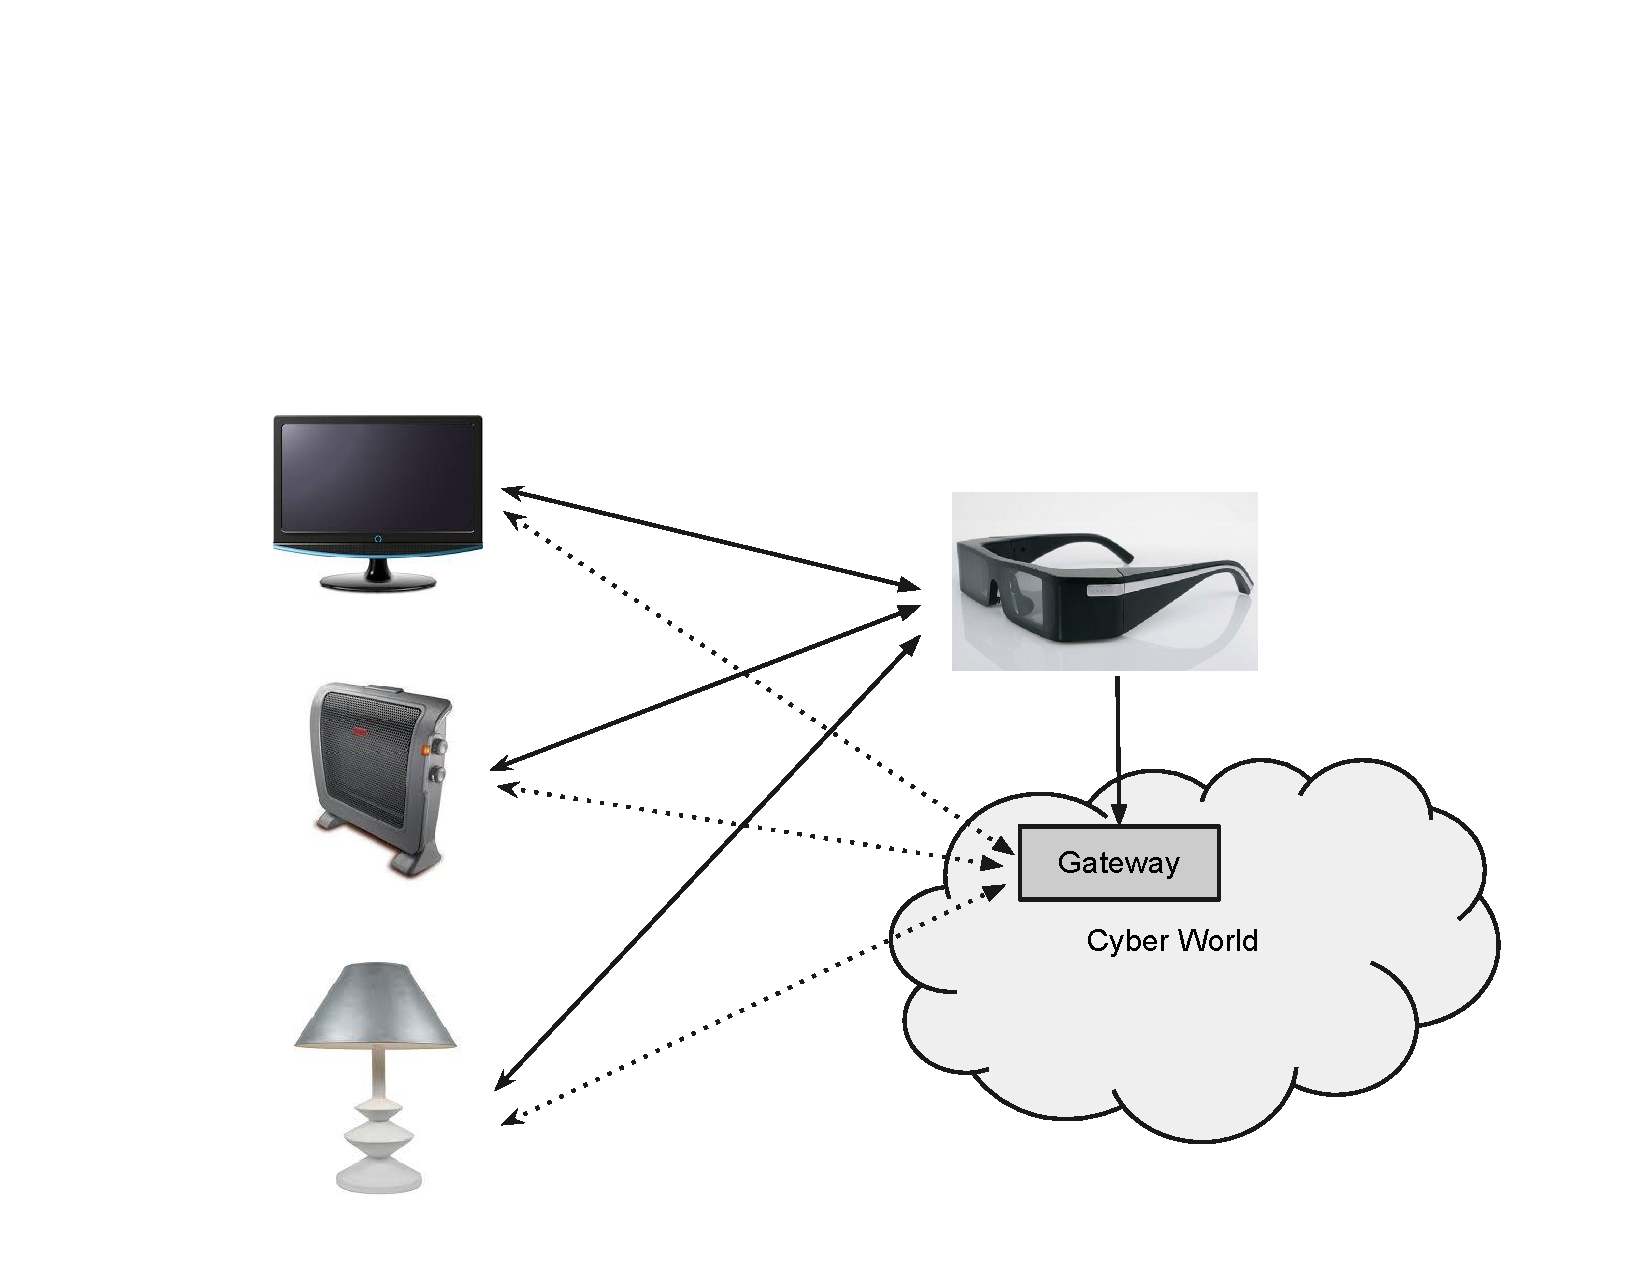
\includegraphics[width=\linewidth]{../figs/sysarch.pdf}
  \caption{System Architecture}
  \label{fig:sysarch}
\end{figure}

The dotted lines show some existing approaches that seek to provide access to physical objects through gateways from the broader Internet. In our project, we focus on the solid lines where the users can interact with them directly. Also as has been pointed out in the requirements, the fall-back scheme for complicated tasks are enabled by the communication between the glasses and the gateway. Though simple enough, we find it essentially useful to have this architectural figure in mind when considering users' interaction.

% Lessons learned from \cite{Bellotti:2002:MSS:503376.503450} have also guided us in thinking the Five A's when designing novel interaction system. 


%%% Local Variables: 
%%% mode: latex
%%% TeX-master: "main"
%%% End: 


\section{Implementation}
\label{sec:implementation}

In this section, we detail our implementation on Arduino \cite{Arduino} platform. The whole system is comprised of a glass module, numbers of clients, and a gateway, as shown in the architecture figure (Fig.\,\ref{fig:sysarch}) in the last section. We will start from the clients, whose primary tasks are to interface between the Glass and the devices that are attached to it. Then we move on to the implementation of the Glass, which manages user's gesture recognition and communication with the clients. The functionality of the gateway so far is confined to only communicate with the clients, since it's not the primary focus of this project.

\subsection{Clients}
The clients are comprised of a main Arduino board, an IR receiver, an XBee radio, and various actuators. We used Arduino Uno, which has an ATmega328 microcontroller and suffice our purpose in this project. We use off-the-shell IR receivers ({\color{red} confirm it is PNA4602}), which outputs 0V (low) on detection of 38 KHz carrier or 5V (high) otherwise. The XBee radio, accompanied with an XBee modems, takes charge of the communication with the Glass. LEDs are added as an indicator of the state of clients and visual feedback for users. Additional components are subject to the device being attached to. In our current system, we have a relay ({\color{red} need to know relay model}) which can control the AC power plug, and we have a USB connected computer to control video playing. The prototype is shown in Fig.\,\ref{fig:client}.

\begin{figure}
  \centering
  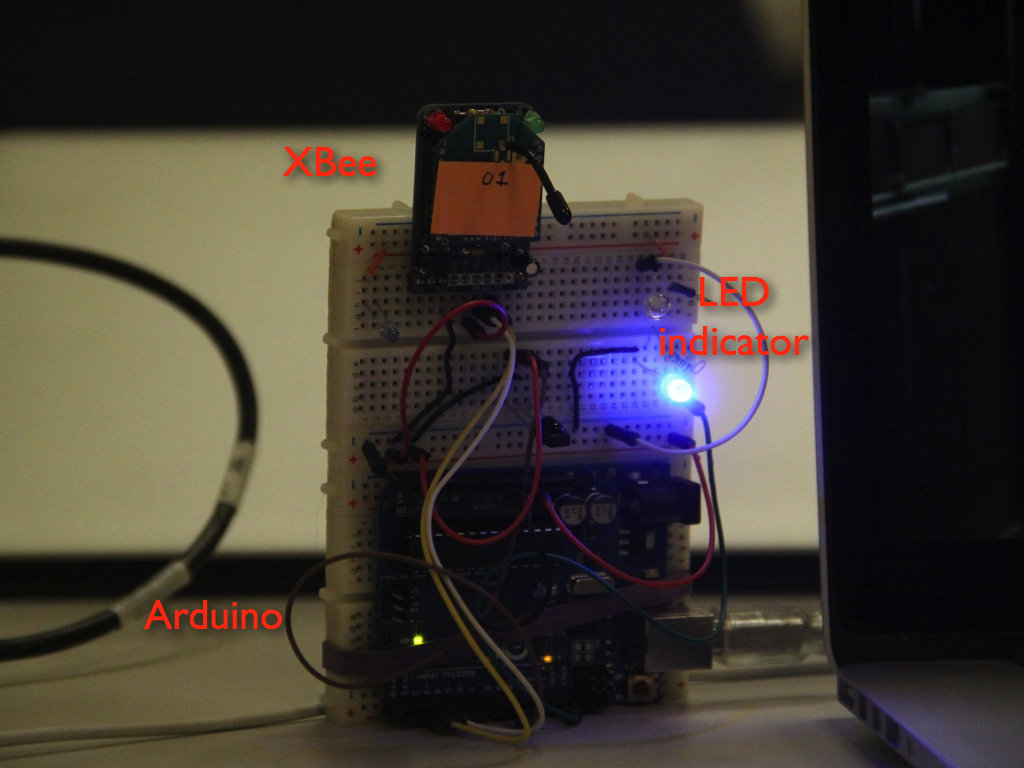
\includegraphics[width=\linewidth]{../figs/client.png}
  \caption{Prototype of the clients}
  \label{fig:client}
\end{figure}

The main function of the client is to respond IR signal and communicate with the Glass to receive commands from the user. Normally, the client stays in {\it IDLE} mode. When it receives an IR signal, suggesting that the user could be interested in interacting with it, the client responds with an XBee acknowledgement and goes into {\it PENDING} state. The glass, after seding the IR, will wait for a certain amoount of time. If there is only one client responding during the wait, the Glass will directly send a connecting message to the only client. When there are multiple clients responding, the Glass will broadcast a verify message with a client ID. The client with a matching ID is called the active client and its LED will blink faster then the others as a visual feedback to the user. After the user decide which one to connect with, the Glass will send out a connecting message. Client turned into {\it CONNECTED} state will be ready to take commands. To summarize the clients' behavior, we have a state machine in Fig.\,\ref{fig:clientFSM} for illustration.

\begin{figure}
  \centering
  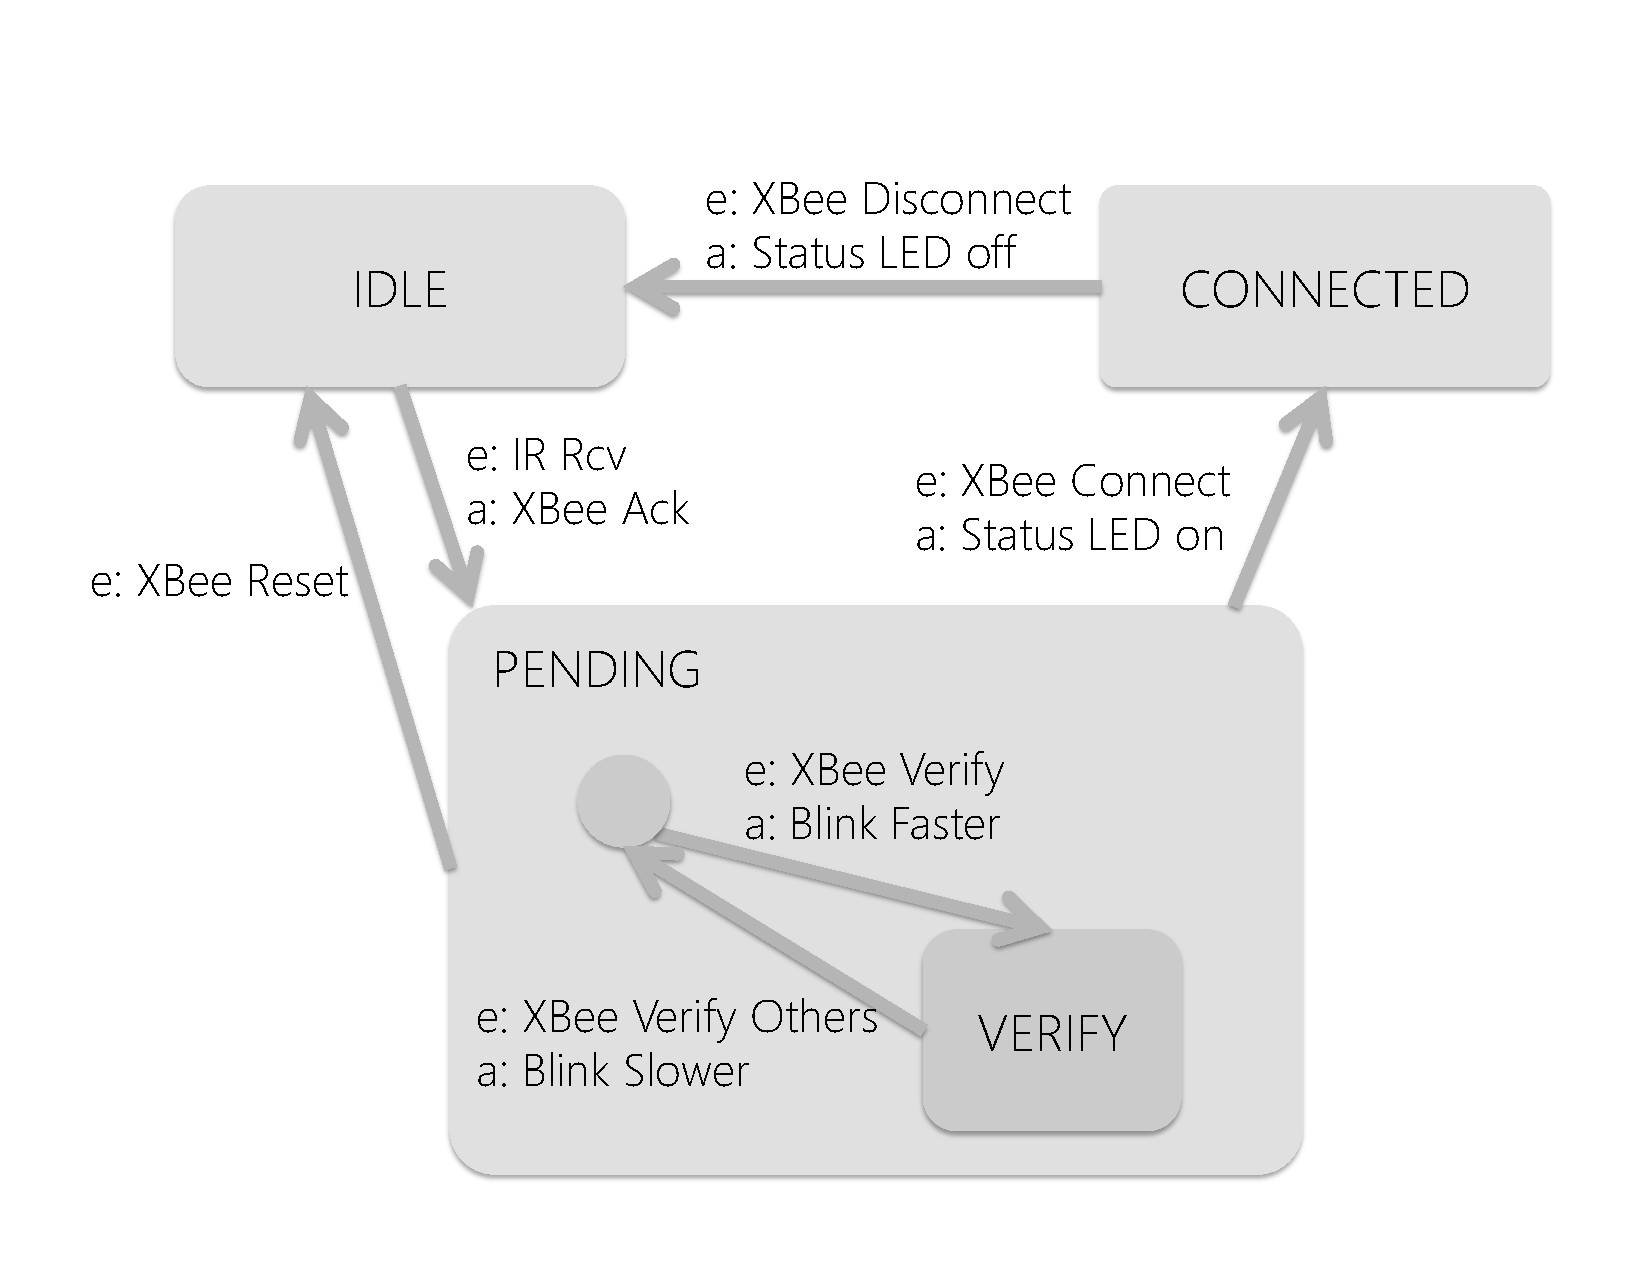
\includegraphics[width=\linewidth]{../figs/clientFSM.pdf}
  \caption{FSM model for client. For each transition, ``e'' stands for event, and ``a'' stands for action}
  \label{fig:clientFSM}
\end{figure}

Within {\it CONNECTED} state, the clients will react differently according to the device it is connected to. In our prototype, we have two different types of devices. The first is a relay, which can control the whole AC power supply. The interface to relay is simply an digital pin. We only need to set it to {\it LOW} or {\it HIGH}. Such command is transmitted remotely from the Glass through XBee using encoded packet. The second tyep is a computer that is used to play video. To send command to the computer, we have a USB adaptor and a python script taking charge of the translation. We use the {\it pyserial} and {\it appscript} library to trigger the play, pause command of an video, and system-wide volume control.

\subsection{Glass}
\label{sec:glass}

The Glass is complicated in two folds. First, we move the complexity of coordinating all clients to the Glass. Second, we have to handle user gesture on Glass. From an engineer perspective, we separate the gesture detection and XBee transmission into two customized library files in Arduino. And only relevant information is sent to the main program. We use the same Arduino Uno and XBee module as the client. An IR emitter is placed within a black tube in order to make the signal a straight beam of light. Then the the tube is attached to the Glass and adjusted in a proper direction. In addition, we have a membrane potentiometer (100 mm long) as the slider to take user's input. After we've put the components onto the Glass, we have the prototype shown in Fig.\,\ref{fig:glass}.

\begin{figure}
  \centering
  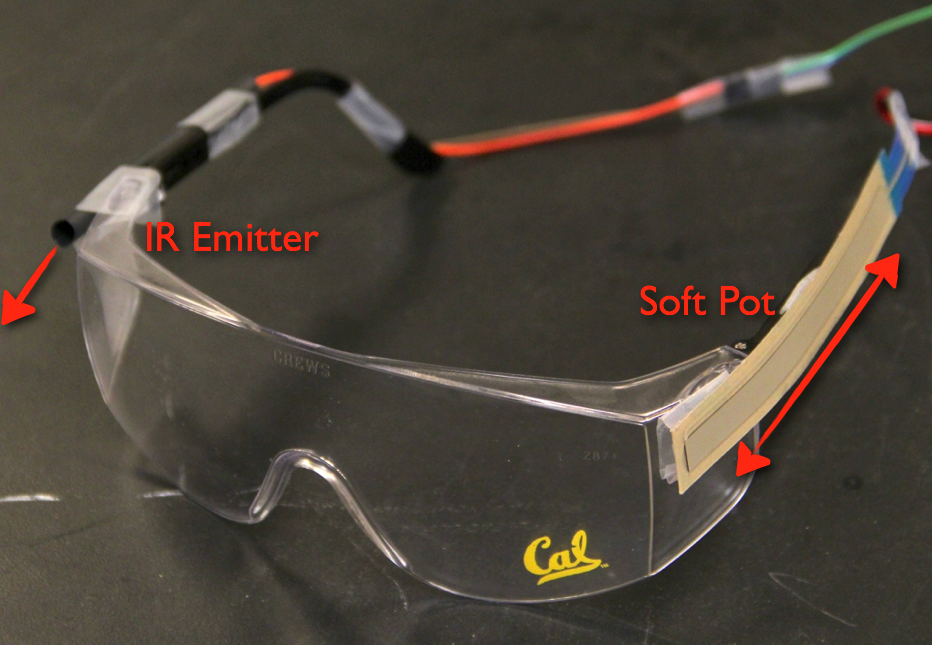
\includegraphics[width=0.85\linewidth]{../figs/glass.png}
  \caption{Prototype of the Glass}
  \label{fig:glass}
\end{figure}


The whole work flow on the Glass is as follows. When the user hasn't shown any interest for interaction, the Glass stays in {\it IDLE} state. When ``tapping'' is detected, the Glass will send a beam of IR signal to inform the devices which are in front of the user. The Glass waited for a specific period of time and count the number of acknowledgement messages responded by the clients. To ensure responsiveness to end user, we set the timer in {\it WAIT} state to be 1 second. When the timer expires, Glass will go to {\it IDLE} if no client has responded, or {\it CONFIRM} if it receives just one message. However, the complicated case is when there are multiple clients that have received the IR signal (because they are near to each other) and responded. Though we expect this scenario rarely happens, there is still chance when the physical devices are put together and it is necessary to differentiate them. In this case, the system goes to {\it VERIFY} state, and sends out corresponding verifying message based on user's gesture. The user can slide back and forth to select the desired target. Once the user confirmed the selection and release his finger, it goes to {\it CONNECTED} state and now the Glass is ready to send out commands. We have the FSM in Fig.\,\ref{fig:glassFSM}.

We've configured the XBee modules such that the Glass can talk in both direction with all clients, while clients cannot talk with each other. In this way, the Glass would serve as master of this personal area network (PAN), whose ID is 4321 in our scenario. 

\begin{figure}
  \centering
  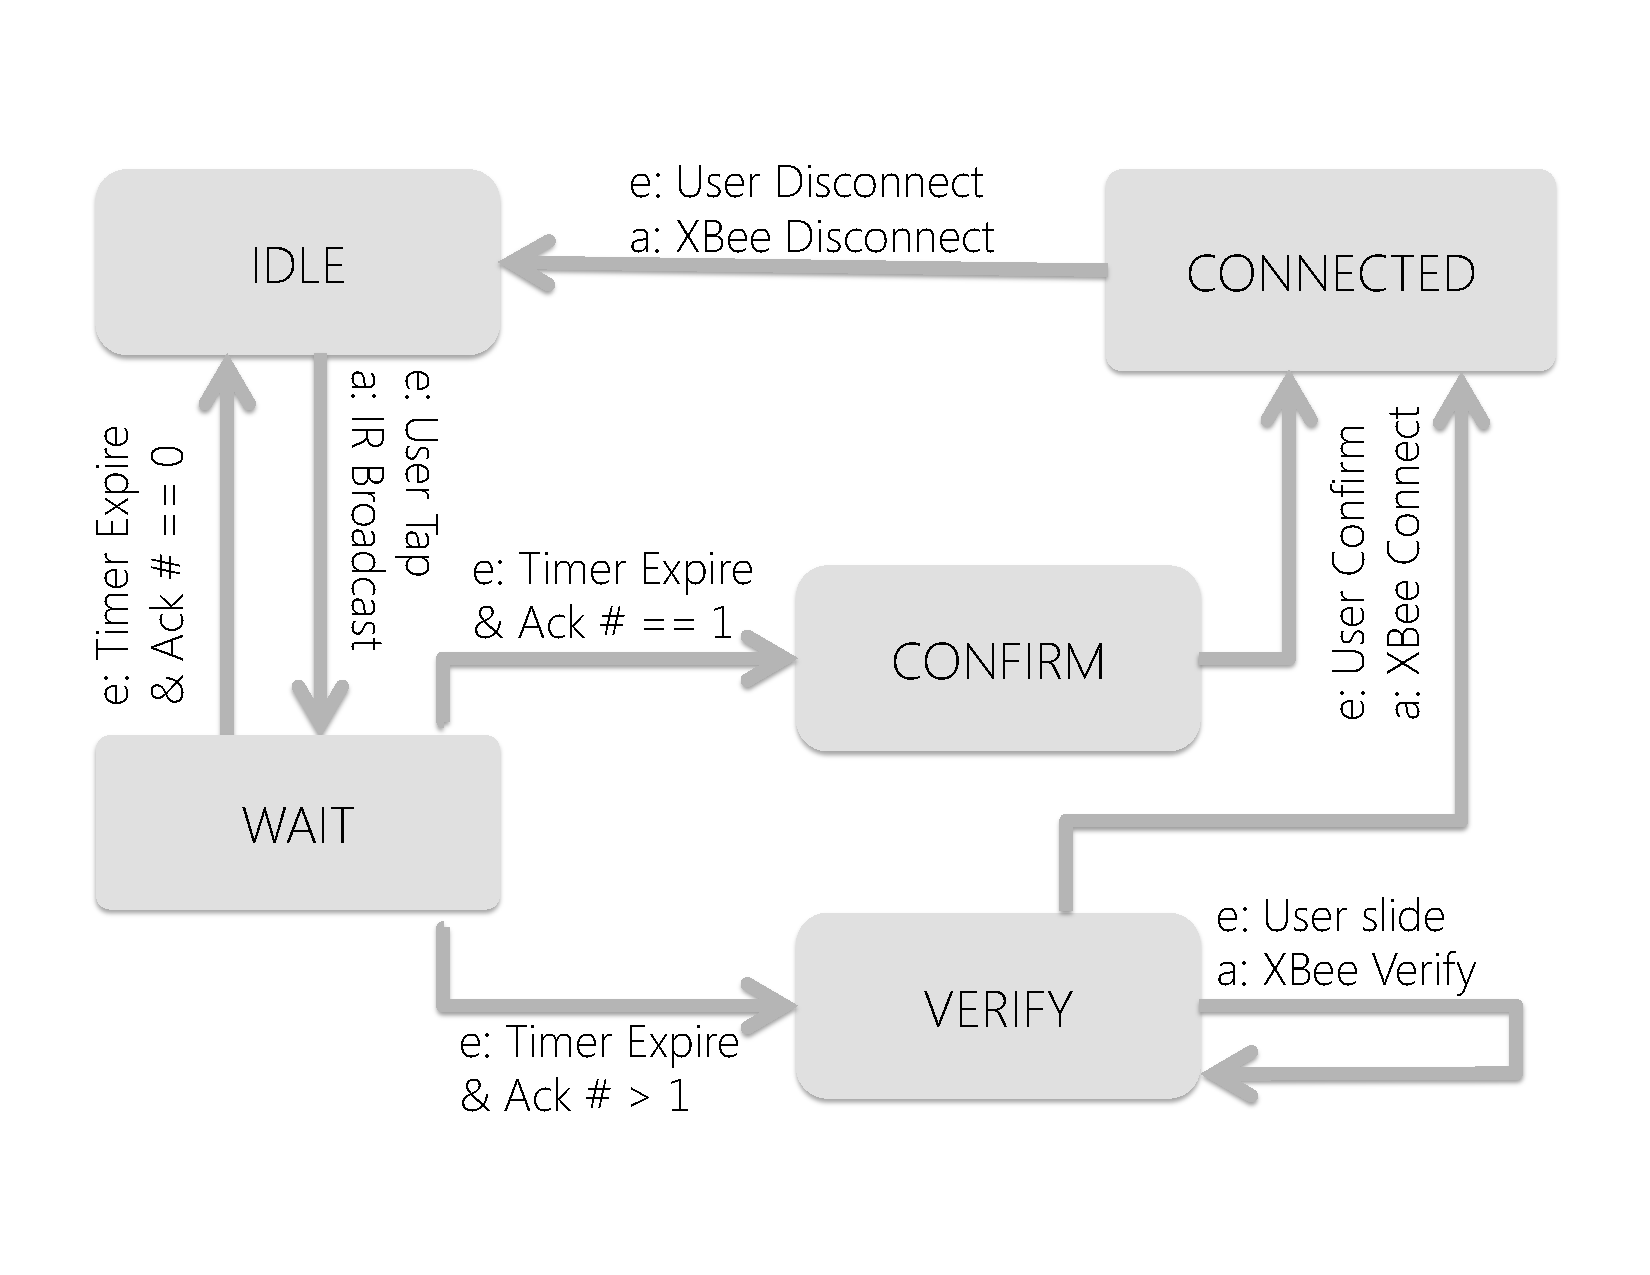
\includegraphics[width=\linewidth]{../figs/glassFSM.pdf}
  \caption{FSM model for Glass. For each transition, ``e'' stands for event, and ``a'' stands for action}
  \label{fig:glassFSM}
\end{figure}

\subsection{Gateway}
\label{sec:gateway}

The gateway provides access to this PAN for computers, and presumably this can be further open to the Internet. Since there have already been many products \cite{NinjaBlocks, Lockitron} that essentially function in this way, we do not spend much time on this aspect in our project. 

For completeness, we wrote a python script that controls a USB XBee adaptor. And this XBee module has the same configuration as the Glass, so it serves as the master of the network. This enables the remote control of the clients.


%%% Local Variables: 
%%% mode: latex
%%% TeX-master: "main"
%%% End: 


\section{Evaluation}
\label{sec:evaluation}

This section we present our work on the evaluation and user study.


%%% Local Variables: 
%%% mode: latex
%%% TeX-master: "uist14"
%%% End: 


\section{Discussion}
\label{sec:discussion}

We discuss a few issues with the system.
%%% Local Variables: 
%%% mode: latex
%%% TeX-master: "uist14"
%%% End: 

\section{Conclusion}
We introduced a novel method for selecting and controlling smart appliances in physical spaces through  infrared targeting based on head orientation. The design takes advantage of the fact that visual attention can express intention, makes it ituitive and helps users remain their focus in the physical world. It addresses the naming and scaling challenges faced by handheld mobile devices. While we present a prototype approach that requires that the user carry additional hardware, all parts can readily be miniaturized and integrated into future head-worn hardware. We also introduced a disambiguation technique in case head orientation is not sufficient to determine a unique target. We characterized our devices performance, arguing that it is matched well to the amount of head movement people can control without strain. A target acquisition study showed that the technique is efficient; a home control scenario showed promise but also limitations when trying to control complex appliances. As our environment continues to be populated by a swarm of sensing and actuation devices, methods to interrogate and control our smart environments may become increasingly important.
%\section{Acknowledgments}
%We thank our user study participants and the a

% \section{Acknowledgments}

\bibliographystyle{abbrv}
\bibliography{reference}

\end{document}
